%%%%%%%%%% Aquí va el código.
\subsection*{Pregunta 3.}

\begin{itemize}  
\item  Dado que un comentario valido en c seria /\textasteriskcentered\textasteriskcentered/
  y en base a la expresión regular brindada esta cadena no es aceptada, no es posible que la
  expresión regular /\textasteriskcentered ([\textasciicircum \textasteriskcentered/]$|$[\textasciicircum \textasteriskcentered]/$|$\textasteriskcentered[\textasciicircum /])$^*$ \textasteriskcentered$^*$ \textasteriskcentered/\\

\item Autómata que acepta comentarios de c :
  \begin{center}
    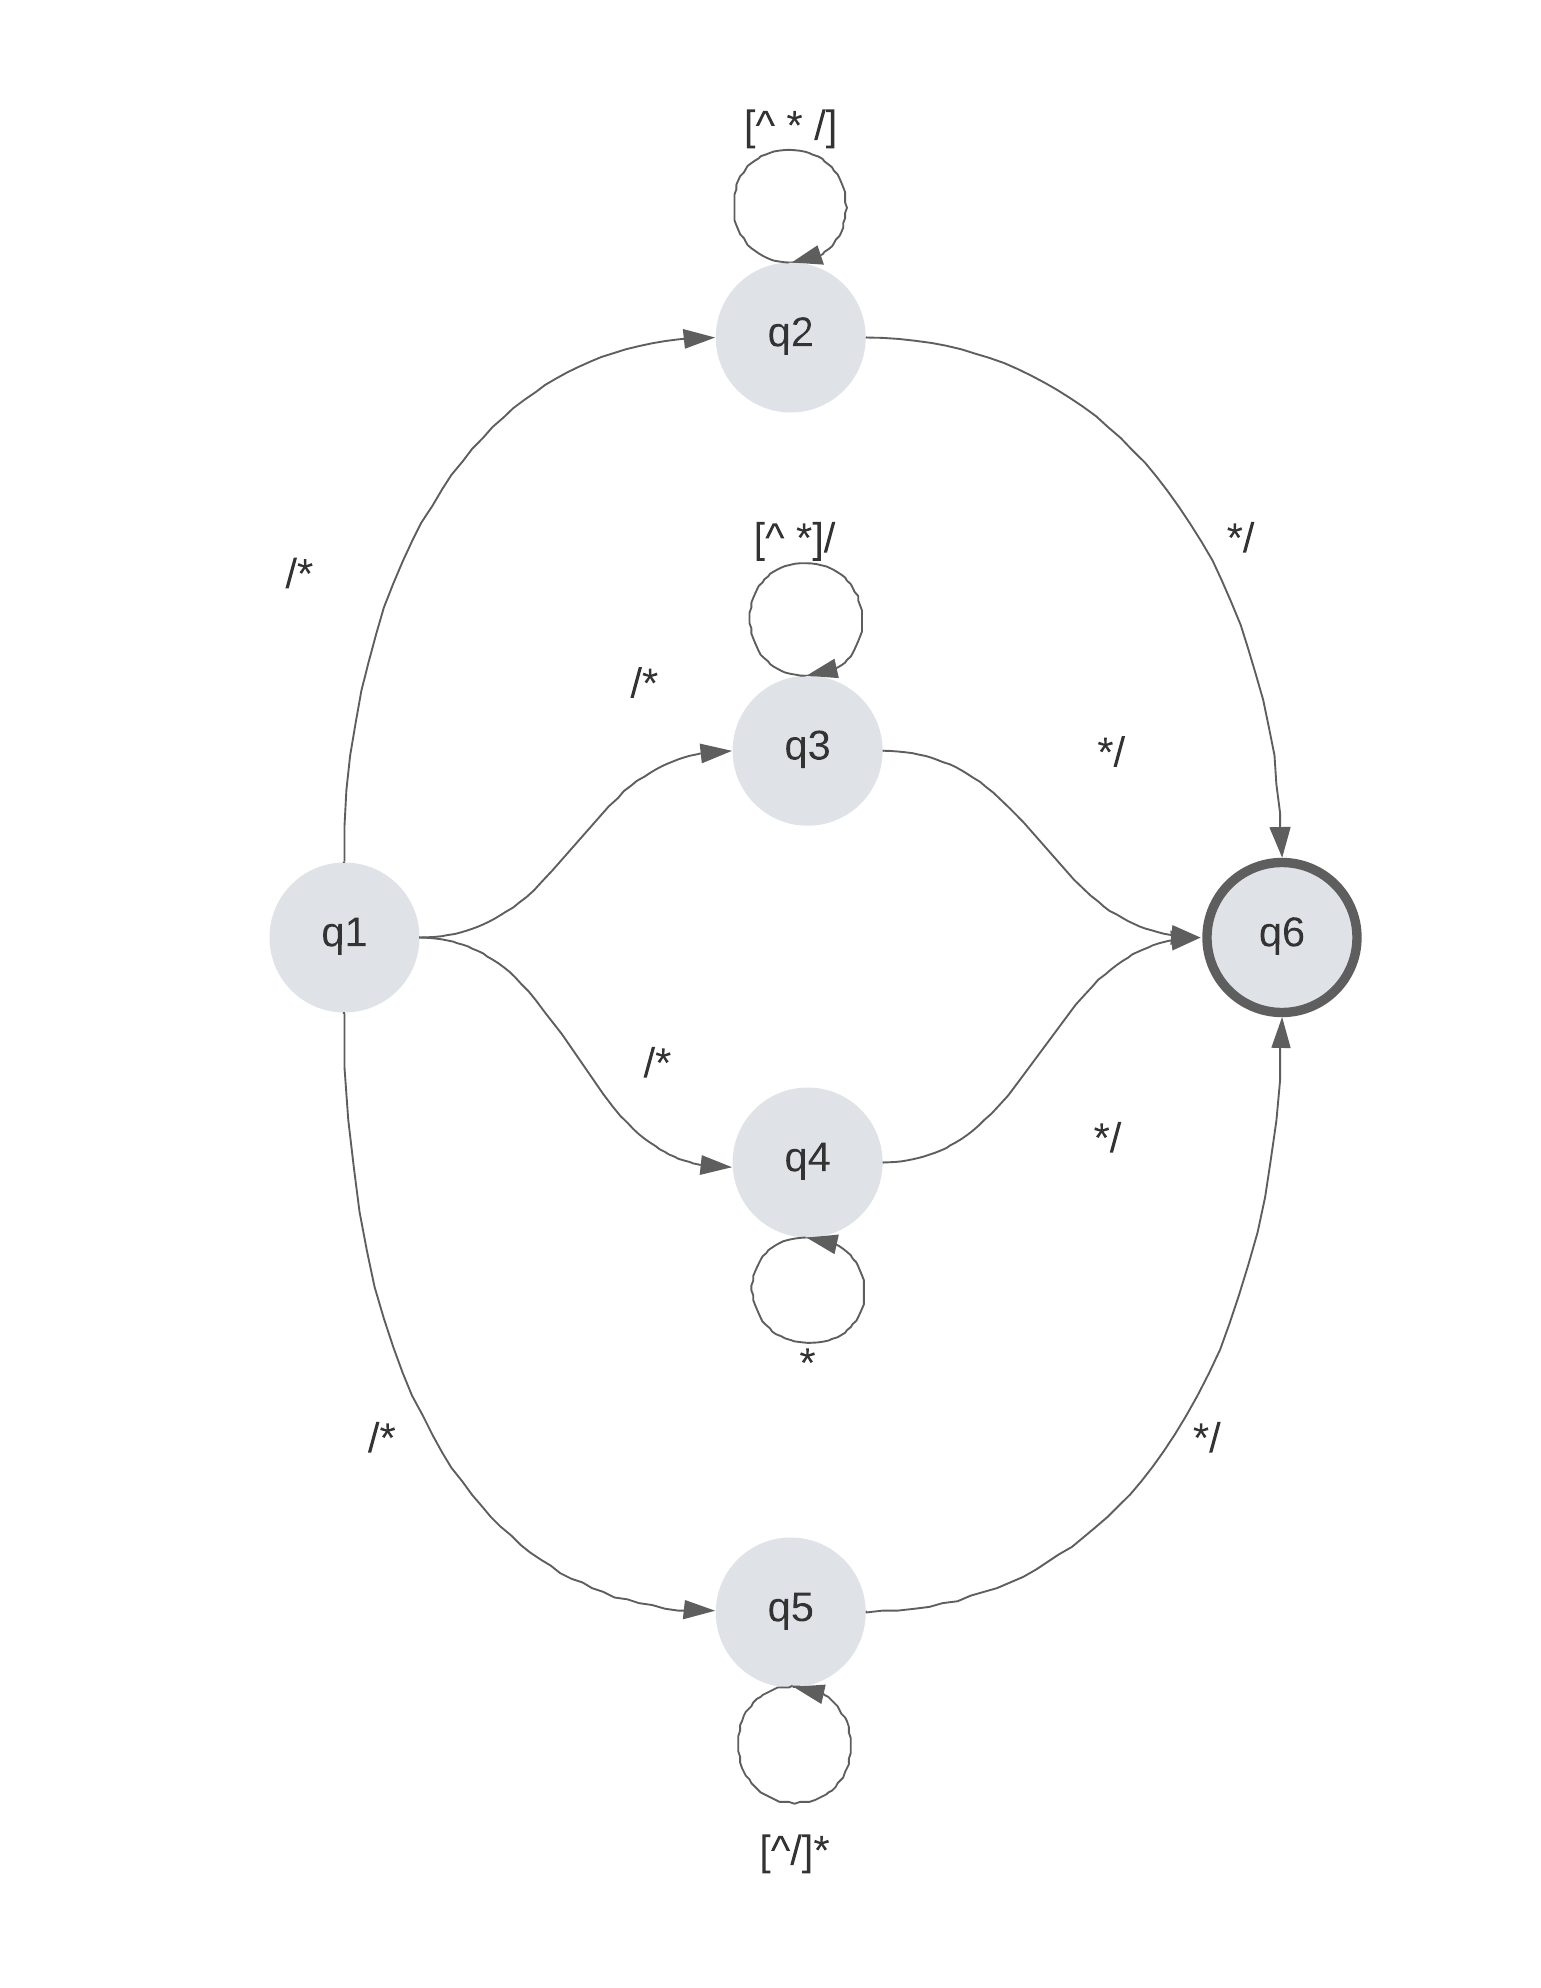
\includegraphics{Comp_Pr3_2.png}
  \end{center}
  
  Expresión regular que corresponde a los comentarios en c
  \[/* \left([\text{\textasciicircum} *\: /] | \left([\text{\textasciicircum} *] /\right)^{\star} |
  \left([\text{\textasciicircum} /] \right)^{\star} | [\text{\textasciicircum} * /]^{+}\right)^{\star} [*]^{\star}*/\]\\
\end{itemize}
